\documentclass[11pt]{extarticle}
\usepackage{apacite, setspace}
\usepackage[margin=1in]{geometry}
%\usepackage{times}
\usepackage{setspace}
\usepackage{float}
\usepackage{subfig}
\usepackage{tikz}
\usepackage{titlesec}
\usepackage{booktabs} % To thicken table lines
\usepackage[shortlabels]{enumitem}
\usepackage{amsthm,amssymb} % for proof 
\usepackage[bottom]{footmisc} %footnote to bottom
\usepackage{amsmath}
\usepackage{cancel}



\usepackage{amsfonts}
% image
\usepackage{graphicx}
\graphicspath{ {img/} }

\usepackage{array}
\newcolumntype{L}[1]{>{\raggedright\let\newline\\\arraybackslash\hspace{0pt}}m{#1}}
\newcolumntype{C}[1]{>{\centering\let\newline\\\arraybackslash\hspace{0pt}}m{#1}}
\newcolumntype{R}[1]{>{\raggedleft\let\newline\\\arraybackslash\hspace{0pt}}m{#1}}


\titlespacing*{\section}
{0pt}{0px}{0px}


% image
\usepackage{graphicx}
\graphicspath{ {img/} }

% for header
\usepackage{fancyhdr}
\pagestyle{fancy}
\lhead{\textbf{ELEC 321 -- Stochastic Signals \& Systems: Homework 2}}
\rhead{Charles Clayton \texttt{\#21518139} }
\cfoot{\thepage} 
\renewcommand{\headrulewidth}{0.4pt}
\renewcommand{\footrulewidth}{0.4pt}
 

 
% for indenting verbating
\usepackage{fancyvrb}

\setlength{\parskip}{\baselineskip}

% automatically convert "" to ``''
\usepackage [autostyle, english = american]{csquotes}
\MakeOuterQuote{"}

\begin{document}

%\pagenumbering{gobble}
\singlespacing



\subsubsection*{Problem 1 Todo: Standard Deviation}

%??? Does this mean standard deviation across different values of m or within the category?

%$$\text{Sensitivity} = P(B|D) = 0.9 \rightarrow P(\overline{B}|D) = 0.1$$ 
%$$\text{Specificity} = P(\overline{B}|\overline{D}) =  0.98 \rightarrow P(B|\overline{D}) = 0.02$$
\begin{enumerate}[(a)]


\item The probability that $m$ additional tests will be taken is the probability that there is a faulty item in the pool. The probability that no items in $m$ are faulty is $(1-p)^m$, so the probability that at least one item in the pool is faulty is $1-(1-p)^m$. Multiply this by $m+1$ to indicate the initial pool test and the subsequent $m$ item tests. 

If no items in the pool are faulty, $(1-p)^m$, then only one test will be taken so the average number of tests per pool is: $$\text{\# tests per pool} = (m+1)(1-(1-p)^m) + 1(1-p)^m$$

And so the cost per pool is: $$X = 5 \left[ (m+1)(1-(1-p)^m) + 1(1-p)^m \right] $$
\begin{table}[H]
\centering
\begin{tabular}{rrcc}
\toprule
\textbf{i} & $\mathbf{m_i}$ & $\mathbf{X_i}$  & $P$ \\
\midrule
1 & 1000 & 5004.8 \\
2 & 500 & 2488.6 \\
3 & 200 & 871.02 \\
4 & 100& 321.98 \\
5 & 50& 103.75 \\
6 & 25& 32.772 \\
7 & 20& 23.209 \\
8 & 10& 9.7809 \\
9 & 8& 8.0902 \\
10 & 5& 6.2252 \\

\bottomrule
\end{tabular}
\end{table}

The mean is the weighted average of all possible values of $X_i$ and their probabilities: $$ \mu = $$  $$ \sigma = $$

\item  So the average number of tests is the average number of tests per pool times the number of pools, $k$: $$T_j \left[ (m+1)(1-(1-p)^m) + 1(1-p)^m \right] $$
\begin{table}[H]
\centering
\begin{tabular}{rrrl}
\toprule
\textbf{j} & $\mathbf{k_j}$ & $\mathbf{T_j} = \mu$ & $\sigma$  \\
\midrule
1 & 1 &  5004.78\\
2 & 2 & 4977.15\\
3 & 5 & 4355.10\\
4 & 10 & 3219.84\\
5 & 20 & 2074.97\\
6 & 40 & 1310.89\\
7 & 50 & 1160.47\\
\textbf{8} & \textbf{100} & \textbf{978.09}\\
9 & 125 & 1011.28\\
10 & 200 & 1245.05 \\
\bottomrule
\end{tabular}
\end{table}



%Probability mass function: $$f(x) = P(X = x)$$
%Distribution function: $$F(x) = P(X \leq x) = \sum_{k=1}^x f(k) $$
%Testing cost: $$X_m = TmP(D)^m$$
%Mean: $$ \mu = E(x) = \sum xf(x)$$
%Variance: $$ \sigma^2 = Var(x) = E \left[(X- \mu)^2 \right] = \sum (x-\mu)^2 f(x) $$


\item The best strategy is where $m = 10$ and $k=100$.

Using the Python (code in Appendix A), I ran 1000 simulations for each pool size to confirm these results, comparing both the simulated and the calculated costs and graphing the two curves. In Figure 1, the \textit{blue} curve\footnote{If this has been printed in black and white, the observation is that the two curves are almost identical.} represents the costs as calculated using the above formula, and the \textit{red} curve represents the cost as determined by averaging the results the simulations.

\begin{figure}[ht!]
\centering
\begin{tabular}{cc}
  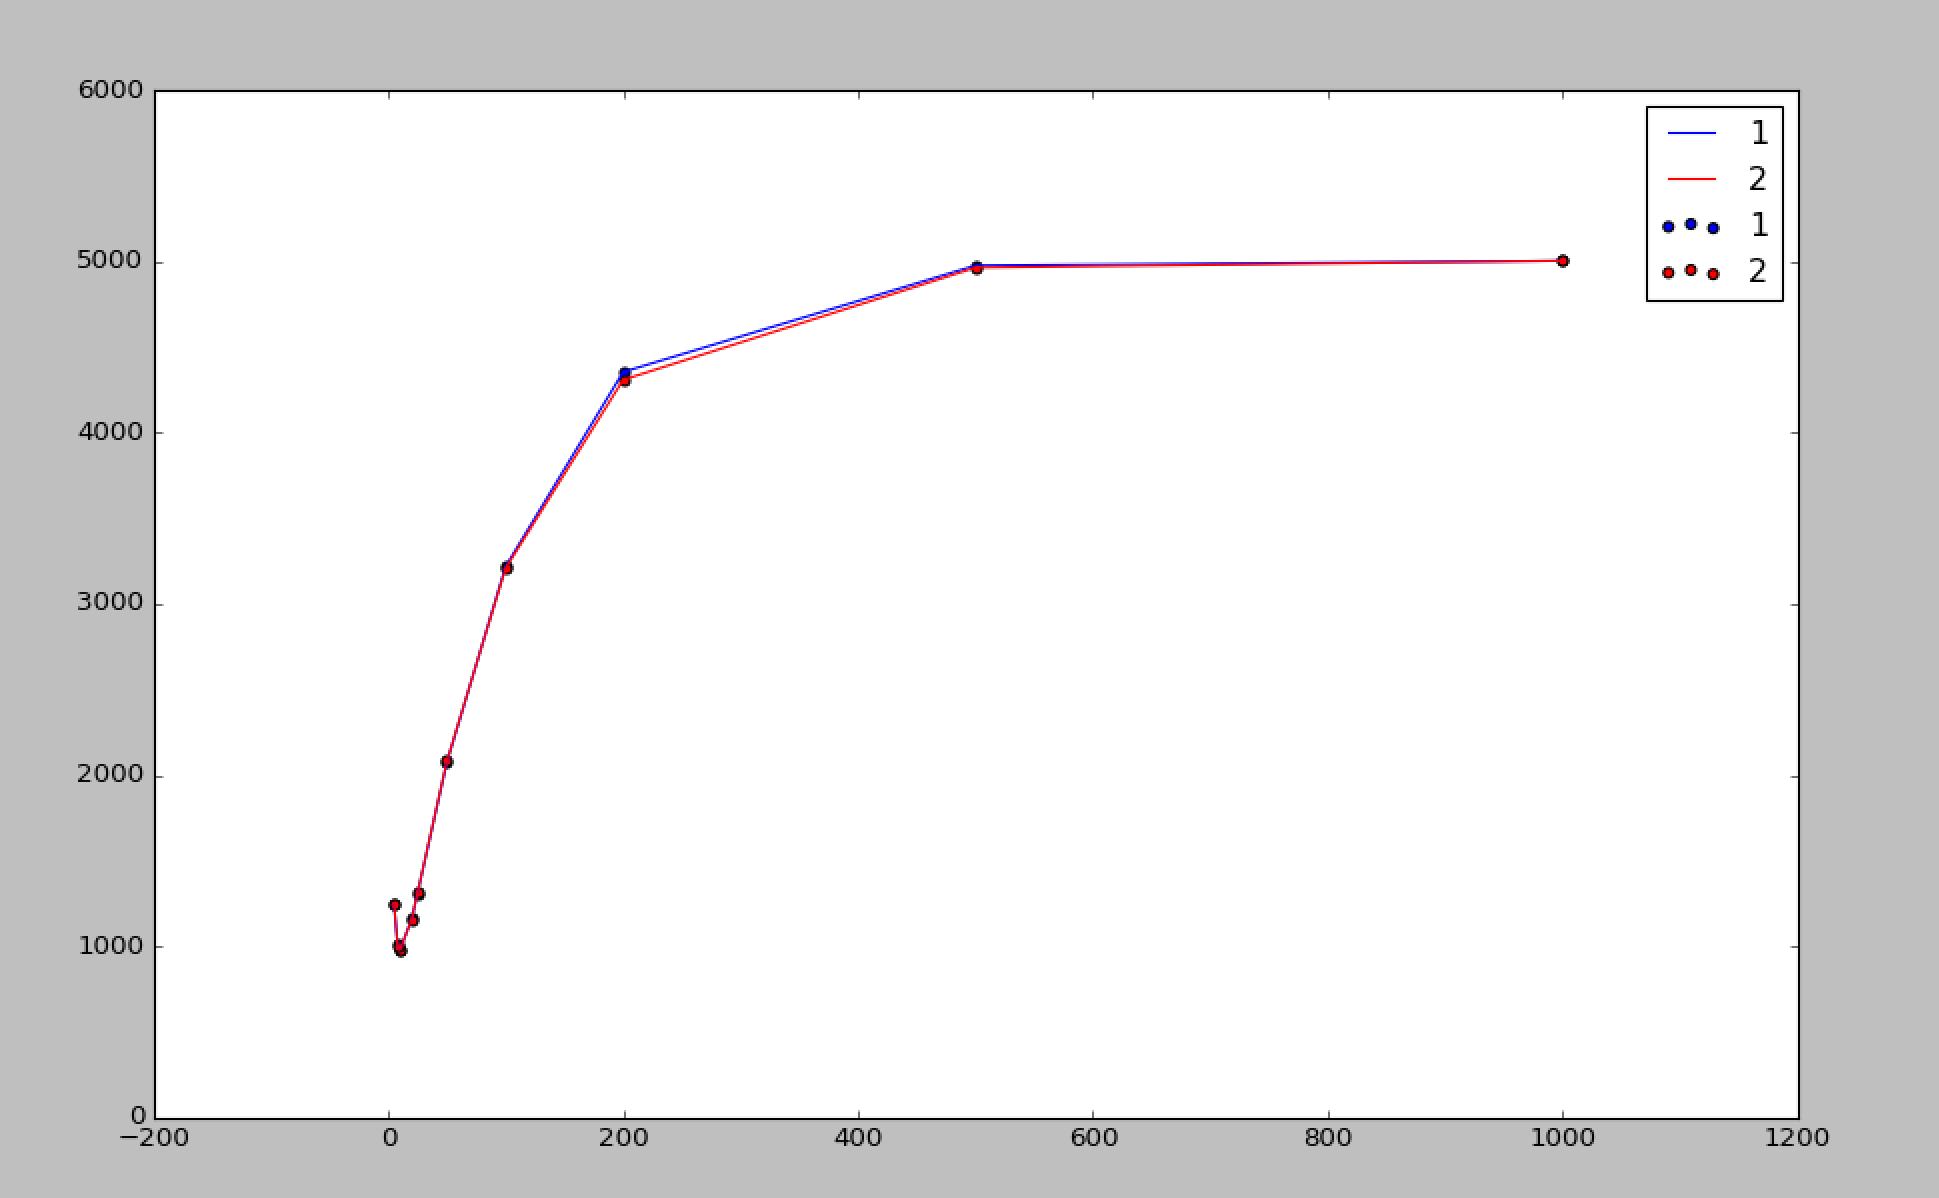
\includegraphics[height=50mm]{P1.png} &   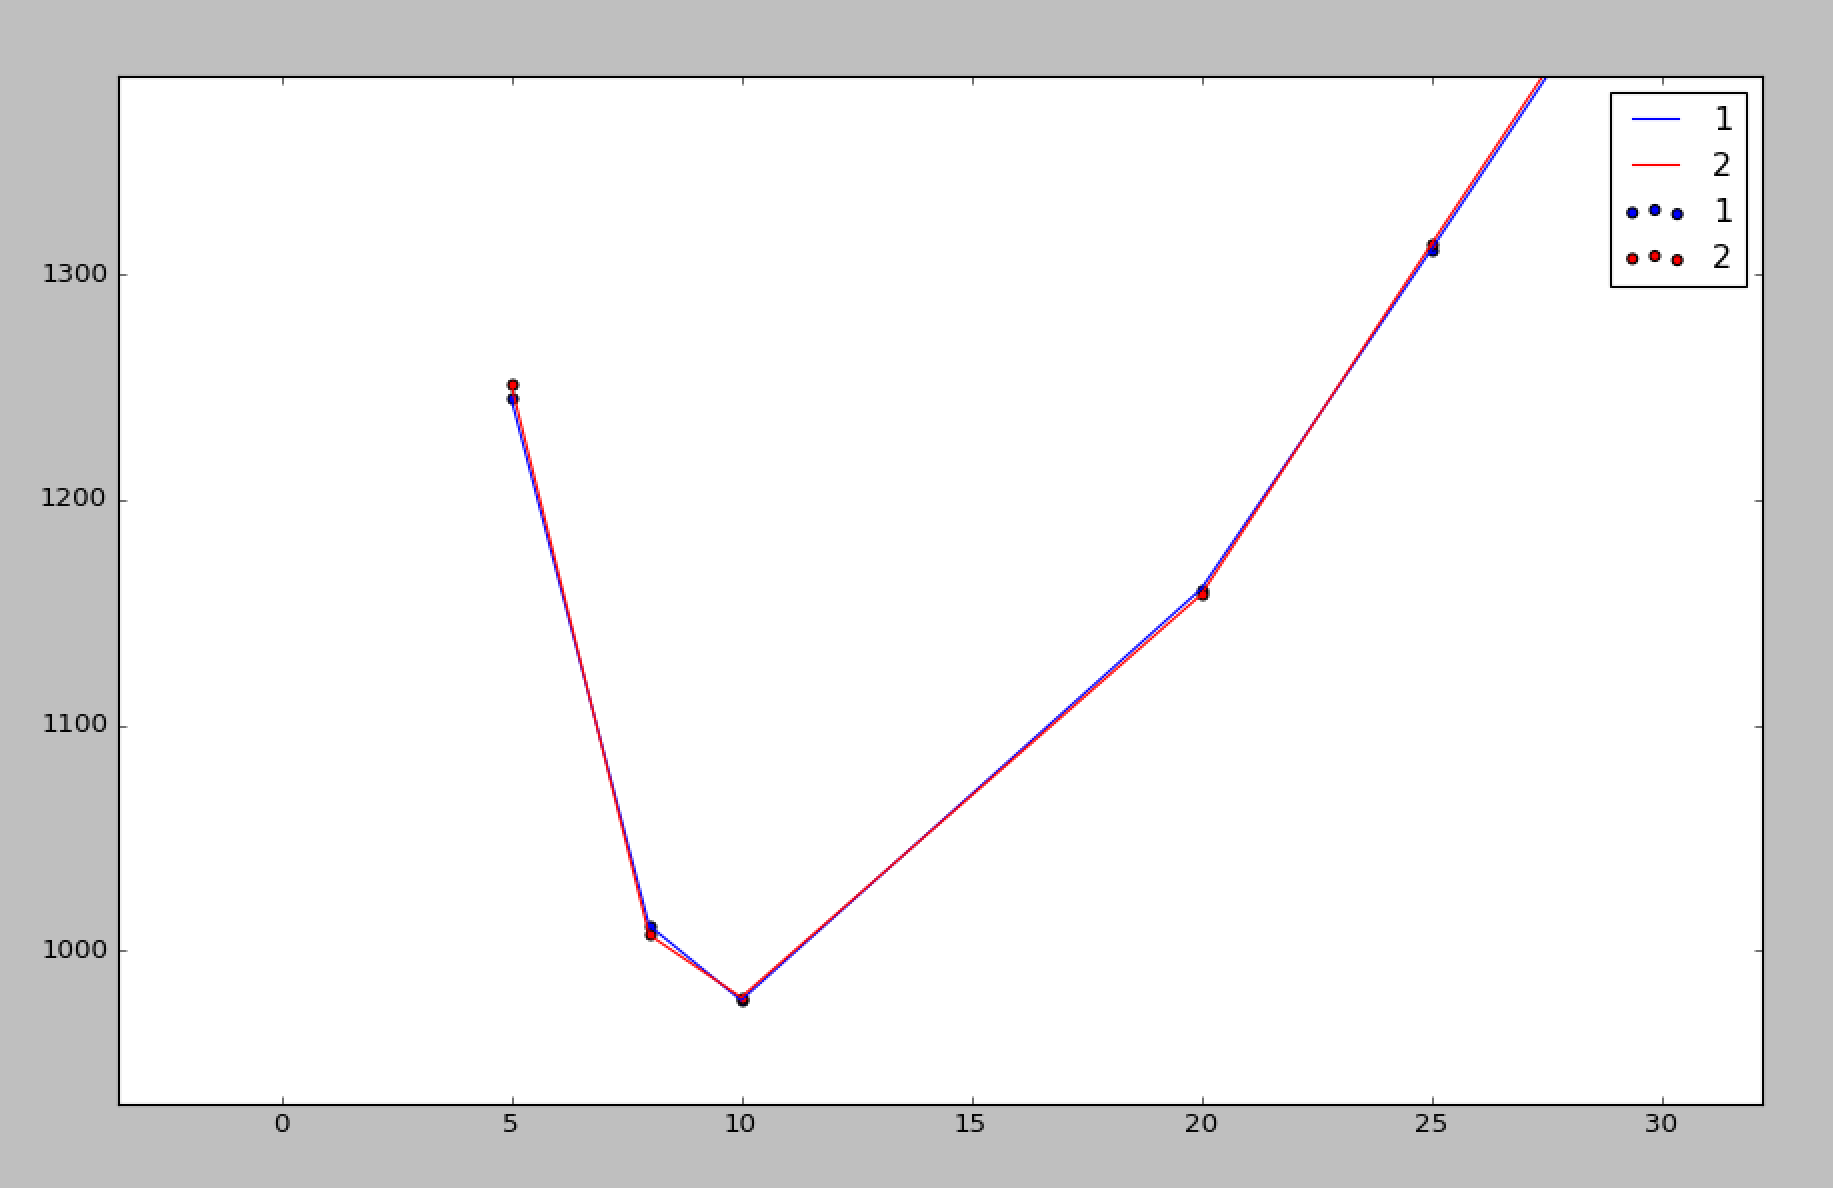
\includegraphics[height=50mm]{P1_2.png} \\
(a) range $m=[0,1000]$ & (b) range $m=[5,30]$ \\[6pt]

\end{tabular}
\caption{Pooling size, $m$ (x-axis) vs. Total cost, $T$ (y-axis)}
\end{figure}


\end{enumerate}

\subsubsection*{Problem 2}

Let $Y$ represent the number of traffic accidents in a given time $[Y \approx P(\lambda)]$ where $\lambda = 5/\text{day} = 35/week = \frac{5}{24}/hour $

\begin{enumerate}[(a)]
\item  For a Poisson distribution: $$\mu = \sigma^2 = \lambda = 35/week $$


\item $$P(X > 40) = 1 - \sum_{i=0}^{40} P(X = i) = 1 - \sum_{i=0}^{40} \frac{e^{-35}(35^i)}{i!} = \boxed{0.17506}$$

%\item $$P(X > 40) = 1 - \int_{i=0}^{40} P(X = i) = 1 - \int_{i=0}^{40} \frac{e^{-35}(35^i)}{i!} = \boxed{0.19689}$$


\item The probability of waiting less than four hours is the same as the probability that an accident happens in the 0$th$, 1$st$, 2$nd$, or 3$rd$ hour.


% $$ P(X < 4) = P(X=0) + P(X=1) + P(X=2) +  P(X=3)  $$
% $$ = \sum_{i=0}^3 \frac{e^{-\frac{5}{24}} \left( \frac{5}{24} \right)^i}{i!} = 0.99993 $$


% Since there are $5/24 = 0.2083$ accidents per hour, then there is one accident every $24/5 = 4.8$ hours, so this seems incorrect.

% It was unclear to me whether I should start counting from the 0$th$ hour or the $1st$ hour, so as before I simulated the situation in Python to compare my answers.

% $$ P(X < 4) = \int_{t=0}^4 \frac{e^{-\frac{5}{24}}\left( \frac{5}{24} \right)^i}{i!} dt = 0.52048$$


 $$ P(X < 4) = \int_{0}^4 \frac{5}{24} e^{-\frac{5}{24}t} dt = 1-e^{-\frac{5}{6}} = \boxed{0.5654}$$
 



\item $$ \frac{n}{\lambda} = \frac{4}{5/24} = \boxed{19.2 \text{\ hours}} $$

\end{enumerate}
 
\subsubsection*{Problem 3}

Where $U$ is a uniform random variable on the interval (0, 1) and $ X = -\ln(1-U)/\lambda $

\begin{enumerate}[(a)]
\item \begin{proof}

%Notice the domain of X is $(-\infty,1)$ so $F_X(x) = 0$ for $x \geq 1$.

%For $x < 1$: $$ F_X(x) = P(X \leq x) = P \left( - \frac{\ln(1-U)}{\lambda} \leq x \right) = P( U \geq 1-e^{-\lambda x} ) = 1 - F_U(1-e^{-\lambda x} ) $$

%Since $U$ is uniform, then $F_U(x) =x $, so: $$ F_X(x) = 1 - (1-e^{-\lambda x} ) = e^{-\lambda x}$$

%For a uniform distribution:
%$$f(X) = \begin{cases}
%		0 & x \leq \alpha \\
%		1/(\beta - \alpha) & \alpha < x < \beta \\
%		0 & x \geq \beta \\
%	\end{cases}$$

%$$F_X(x) = \begin{cases}
%		0 & x \leq \alpha \\
%		\frac{1}{\beta - \alpha} \int_{\alpha}^{x} dt = \frac{x-\alpha}{\beta-\alpha} & \alpha < x < \beta \\
%		1 & x \geq \beta \\
%	\end{cases}$$
	
%$$ \mu = \frac{\alpha + \beta}{2},\  \ \ \mu_2 = \frac{\beta^2 + \alpha^2 + \alpha \beta}{3}   $$	

%$$ \sigma^2 = \mu_2 - \mu^2 = \frac{(\beta - \alpha)^2}{12}	$$
	
%Where $\alpha = 0$ and $\beta=1$:

%$$F_X(x) = \frac{x-1}{1-0}$$


Notice that the range of $X$ is $(-\infty, 1)$, so for $x > 1$: $$ F_X(x) = 0$$

For $x \leq 1$: \begin{equation} 
\begin{split} F_X(x) & =  P(X \leq x) \\ 
& = P( -\ln(1-U)/\lambda \leq x)  \\
& = P(U \leq 1-e^{-\lambda x}) \\
& = F_U(1-e^{-\lambda x}) 
\end{split}
\end{equation}
 Since $U$ is Unif$(0, 1)$, then $ F_U(u) = u,\ 0 \leq u \leq 1 $, so: $$ \boxed{F_X(x)  = 1- e^{-\lambda x}} $$ 

$$ f_X(x) = \frac{\partial}{\partial x} F_X(x) = \lambda e^{- \lambda x} $$

% Blah: $$ E(X) = \frac{1}{\lambda} $$ $$ Var(X) = \frac{1}{\lambda^2} $$

Mean: $$ \mu = E(X) = \int_{0}^{\infty} x f_X(x) dx = \int_{0}^{\infty} x \lambda e^{- \lambda x} dx  $$ 
$$ =  -x e^{-\lambda x}\Big|_0^\infty + \frac{-1}{\lambda} e^{-\lambda x} \Big|^\infty_0 = \boxed{\frac{1}{\lambda} } $$

Variance: $$ \sigma^2 = Var(X) = E(X^2) - E(X)^2  $$ $$=  \left( \int_{0}^{\infty} x^2 \lambda e^{- \lambda x} dx  \right) - \left( \frac{1}{\lambda} \right)^2 $$ 

$$ = \left( \frac{2}{\lambda^2} \right)  - \left( \frac{1}{\lambda} \right)^2 = \boxed{\frac{1}{\lambda^2}} $$


\end{proof}

\item $$Y = e^{\lambda X} =  e^{-\lambda \ln(1-U)/\lambda} = e^{-\ln(1-U)} = \frac{1}{1-U}$$

Notice that the range of $Y$ is $(-\infty, 1)$, so for $y > 1$: $$ F_Y(y) = 0$$

For $x \leq 1$: \begin{equation} 
\begin{split} F_Y(y) & =  P(Y \leq y) \\ 
& = P \left( \frac{1}{1-U} \leq y \right)  \\
& = P \left( U  \leq \frac{y-1}{y} \right)  \\
& = F_U \left( \frac{y-1}{y} \right)
\end{split}
\end{equation}
 Since $U$ is Unif$(0, 1)$, then $ F_U(u) = u,\ 0 \leq u \leq 1 $, so: $$ \boxed{F_Y(y)  = \frac{y-1}{y} } $$ 

$$ \boxed{f_Y(y) = \frac{\partial}{\partial x} F_Y(y) = \frac{1}{y^2}} $$

\end{enumerate}

\subsubsection*{Problem 4 (Incomplete)}

Let $Z$ be the standard normal variable with density:$$ \varphi(z) =  f(z) =  \frac{1}{\sqrt{2 \pi}} e^{-(z^2/2)} $$

\begin{enumerate}[(a)]
\item \begin{proof} \begin{align*}
I^2  = & \frac{1}{2\pi} \int_{-\infty}^{\infty} \int_{-\infty}^{\infty} e^{-(x^2 + y^2)/2}\ dxdy \\
 =& \frac{1}{2\pi} \int_{-\pi}^{\pi} \int_{0}^{\infty} e^{-r^2/2}\ r dr d\theta  \\
  =& \frac{1}{2\pi} \int_{0}^{2\pi} \int_{0}^{\infty} e^{-r^2/2}\ r dr d\theta \\
  =& \frac{1}{2\pi} 2\pi  \Big[ -e^{-r^2/2}\ \Big|_0^\infty \Big] \\
  =& \frac{1}{2\pi} 2\pi [0 - (-1)] \\
  =& 1
\end{align*}

%$ \frac{1}{\sqrt{2\pi}} \int_{-\infty}^{\infty}  e^{-(z^z/2)}  dz $

Since $I^2 = 1$, then $I = \pm 1$. Since $e^{-(z^2/2)} > 0$ for all $z$, then $I=1$, as required. \end{proof}

\item $$\varphi'(z) = -z \varphi(z) $$ $$z \varphi'(z) = -z \varphi(z) $$

\begin{proof} Mean: \begin{align*} \mu = E(Z) & = \int_{-\infty}^{\infty} z f(z) dz \\
& =  \int_{-\infty}^{\infty} z \frac{1}{\sqrt{2 \pi}} e^{-(z^2/2)} dz\\
& =  \int_{-\infty}^{0} z \frac{1}{\sqrt{2 \pi}} e^{-(z^2/2)} dz + \int_{0}^{\infty} z \frac{1} {\sqrt{2 \pi}} e^{-(z^2/2)} dz & add more detail\\
& = \frac{-1}{2\pi} + \frac{1}{2\pi}\\
& =  0 \end{align*} \end{proof}

\begin{proof} Variance: \begin{align*} \sigma^2 = Var(Z) =  E(Z^2) - \cancelto{0}{E(Z)^2} & = E(Z^2) \\
& =  \int_{-\infty}^{\infty} z^2 f(z) dz\\
& =  \int_{-\infty}^{\infty} z^2 \frac{1}{\sqrt{2 \pi}} e^{-(z^2/2)} dz & Add more detail\\
& =  1 \end{align*} \end{proof}


\end{enumerate}
\subsubsection*{Problem 5}

Suppose the lifetime $Y$ of a system has failure rate $h(y) = 2y$, $y>0$.

\begin{enumerate}[(a)]
\item Assuming $y$ represents time, then the failure rate increases with time so the system gets weaker as it ages.
\item $$F_Y(x) = 1 - \exp \left( -\int_0^x h(y)\ dy \right) = 1 - \exp \left( -\int_0^x 2y\ dy \right) = \boxed{ 1 - e^{-x^2} }$$

$$ f_Y(x) = \frac{\partial}{\partial x} \left( 1 -e^{-x^2} \right) = \boxed{ 2x e^{-x^2} } $$

\item $$F_Y(m) = \frac{1}{2}  = 1 - e^{-m^2} \rightarrow m = \pm \ln{2}$$ $$ \boxed{m=0.83255} $$

\end{enumerate}

\subsubsection*{Problem 6 (Am I allowed to use code here?)}

$$ X \sim N(5, \sigma^2 )$$
$$F(x) = P(X \leq x) =  \Phi \left( \frac{x - 5}{\sigma} \right)$$

Determine $\sigma$ where:  $$ \frac{1}{100} = 1 - P(-0.02 \leq X \leq 0.02) = 1 - \left[ \Phi \left(\frac{0.02}{\sigma} \right) - \Phi \left( \frac{-0.02}{\sigma} \right) \right] = 1 - \left[ 2 \Phi(0.02)-1 \right] $$ 
 $$ \frac{99}{100} = P(-0.02 \leq X \leq 0.02) =  \Phi \left(\frac{0.02}{\sigma} \right) - \Phi \left( \frac{-0.02}{\sigma} \right)  = 2 \Phi \left( \frac{0.02}{\sigma} \right) -1  $$ 

Doing a direct search with the code in Appendix C to solve for $\sigma$, when $\boxed{\sigma < 0.007764489}$ at most 1\% of the ball bearings are out-of-spec.

\subsubsection*{Problem 7 (What does actual temperature of the medium mean?)}

$\sigma=0.1\mu$, $\sigma^2 =  0.01\mu^2$.

$$ X \sim N(\mu, 0.01\mu^2 ) $$ 
$$ 0.95 = P(-0.1 \leq X \leq 0.1) = 2\Phi \left( \frac{0.1}{0.1\mu} \right)-1 $$

Doing a direct search with the code in Appendix D to solve for $\mu$, when $\boxed{\mu < 0.51021345}$ the probability is larger than or equal to $0.95$ that the temperature reading is within 0.1.

\subsubsection*{Problem 8 (Not Started)}

Show $U = F_X(X)$ is uniform on interval (0, 1) where $X$ is continuous and has invertible cdf $F_X(x)$.

Call $Q_X(x)$ a quantile of $X$. If $F_X$ is invertible, then $F_X^{-1}(x) = Q_X(x)$.

Given a uniform variable $U$ on the interval [0, 1] and an invertible cdf $F_X$, then the random variable $X=F_X^{-1}(U)$ has distribution $F$.

Since $F$ is continuous, then $F$ is invertible since it is continous and strictly increasing. .

\subsubsection*{Problem 9 (Not Started)}



\subsubsection*{Problem 10 (Unsure)}


\textbf{Using Python:
}\begin{verbatim}n = 10000000
x1 = numpy.random.normal(loc=90,  scale=10, size=n)
x2 = numpy.random.normal(loc=100, scale=12, size=n)
x3 = numpy.random.normal(loc=110, scale=14, size=n)
v  = x2 - 1/2*(x1+x3)
print(len([i for i in v if -9 <= i <= 9])/n)

>>> 0.4578041
\end{verbatim}

\textbf{Using R:
}\begin{verbatim}n <- 10000000
x1 <- rnorm(n, mean=90,  sd=10)
x2 <- rnorm(n, mean=100, sd=12)
x3 <- rnorm(n, mean=110, sd=14)
v  <- x2 - 0.5*(x1+x3)
sum(-9 <= v & v <= 9)/n

> [1] 0.457829
\end{verbatim}

$$ P \left( -9 \leq X_2 - \frac{1}{2} (X_1 + X_3 ) \leq 9 \right) \approx  \boxed{0.4578}$$ %$$P \left( X_2 - \frac{1}{2} (X_1 + X_3 ) \leq 9 \right) -  P \left(  X_2 - \frac{1}{2} (X_1 + X_3 ) \leq -9 \right)   $$


\subsubsection*{Problem 11 (How do we get $x-\mu=\epsilon$???}

\begin{enumerate}[(a)]

\item \begin{proof}
$$P( |X - \mu| \leq \epsilon) \geq 1 - \frac{\sigma^2}{\epsilon^2},\ \text{for all}\ \epsilon > 0$$

Where $X$ is a random variable with mean $\mu$ and variance $\sigma^2$, and $\epsilon > 0$: \begin{equation*} \begin{split} \sigma^2 = & \int_{-\infty}^{\infty} (x-\mu)^2 f(x) dx \\  
\end{split} 
\end{equation*}
As given: \begin{equation*} \begin{split}
\sigma^2 \geq & \int_{-\infty}^{\mu-\epsilon} (x-\mu)^2 f(x) dx + \int_{\mu+\epsilon}^{\infty} (x-\mu)^2 f(x) dx \\ 
\end{split} 
\end{equation*}
Factoring: \begin{equation*} \begin{split} \sigma^2 \geq & (x-\mu)^2 \Big( \int_{-\infty}^{\mu-\epsilon} f(x) dx + \int_{\mu+\epsilon}^{\infty} f(x) dx \Big) 
\end{split} 
\end{equation*}
By CDF definition: %\begin{equation*}
%\begin{split}
%= & (x-\mu)^2 \Big( F(\mu-\epsilon) + F(\mu+\epsilon ) \Big) 
%\end{split}
%\end{equation*}
%By CDF definition again: 
\begin{equation*}
\begin{split}
\sigma^2 \geq & (x-\mu)^2 \Big( P(X \leq \mu-\epsilon) + P(X \geq \mu+\epsilon ) \Big) \\
\sigma^2 \geq & (x-\mu)^2 \Big( P( X - \mu \leq -\epsilon) + P(X - \mu \geq \epsilon ) \Big) \\
\sigma^2 \geq & (x-\mu)^2 \Big(  P(|X - \mu| \geq \epsilon ) \Big) \\
\end{split} 
\end{equation*}

Dividing by $(x-\mu)^2$: \begin{equation*} \begin{split} 
P(|X - \mu| \geq \epsilon )   \leq \ &\frac{\sigma^2}{(x-\mu)^2}   \\
 P(|X - \mu| \leq \epsilon )   \geq \  & 1 - \frac{\sigma^2}{(x-\mu)^2}  \\
\end{split} 
\end{equation*}

Since $x-\mu = \epsilon$ (???): $$  \boxed{ P(|X - \mu| \leq \epsilon )   \leq 1-  \frac{\sigma^2}{\epsilon^2} } $$



\end{proof}

\item \begin{proof} $$ \overline{X} = \frac{X_1 + X_2 + \dots + X_n}{n} $$

So: \begin{align*}E( \overline{X} ) & = E \left( \frac{X_1 + X_2 + \dots + X_n}{n} \right) \\
& = \frac{1}{n} \left( E(X_1) + E(X_2) + \dots + E(X_n) \right) \\
& = \frac{1}{n} \left( \mu_1 + \mu_2 + \dots + \mu_n \right) \\
& = \frac{1}{n} \left( \mu(n) \right) = \boxed{\mu}  
\end{align*} \end{proof}

\begin{proof} $$ \overline{X} = \frac{X_1 + X_2 + \dots + X_n}{n} $$

So: \begin{align*}Var( \overline{X} ) & = Var \left( \frac{X_1 + X_2 + \dots + X_n}{n} \right) \\
& = Var \left( \frac{X_1}{n} +  \frac{X_2}{n} + \dots +  \frac{X_n}{n} \right) \end{align*} 
Since $X_1$, $X_2$, $\dots$ , $X_n$ are independent\footnote{Assuming "independently measured" mean independent}, $Var \left( \sum_{i=1}^n (X_i) \right) = \sum_{i=1}^N Var(X_i)$, so:
 \begin{align*}
Var( \overline{X} ) & = Var \left( \frac{X_1}{n} \right) + Var \left( \frac{X_2}{n} \right) + \dots + Var \left( \frac{X_n}{n} \right) 
\end{align*} 
From $Var(aX) = a^2 Var(X)$: \begin{align*} 
Var( \overline{X} ) & = \frac{1}{n^2} Var(X_1) + \frac{1}{n^2} Var(X_2) + \dots + \frac{1}{n^2} Var(X_n)  \\
& = \frac{1}{n^2} \Big( Var(X_1) + Var(X_2) + \dots +  Var(X_n) \Big)  \\
& = \frac{1}{n^2} \Big( \sigma_1^2 + \sigma_2^2 + \dots +  \sigma_n^2 \Big)  \\
& = \frac{1}{n^2} \sigma^2(n)  = \boxed{ \frac{\sigma^2}{n} } 
\end{align*} \end{proof}
\item \begin{proof}From (a), for all $\epsilon > 0$:
\begin{align*}
P(|X - \mu| \leq \epsilon )  & \leq 1-  \frac{\sigma^2}{\epsilon^2} 
\end{align*}
Substituting $\overline{X}$ for $X$:
\begin{align*}
P(|\overline{X} - E(\overline{X})| \leq \epsilon )  & \leq 1-  \frac{Var(\overline{X})}{\epsilon^2} \\
P(|\overline{X} - E(\overline{X})| \geq \epsilon )  & \leq \ \frac{Var(\overline{X})}{\epsilon^2} 
\end{align*}
From (b), substituting $E(\overline{X}) = \mu $ and $Var(\overline{X}) = \frac{\sigma^2}{n}$:
\begin{align*}
P(|\overline{X} - \mu| \geq \epsilon )  & \leq \ \frac{\frac{\sigma^2}{n}}{\epsilon^2}   \\
P(|\overline{X} - \mu| \geq \epsilon )  & \leq \ \frac{\sigma^2}{n\epsilon^2}   
\end{align*}
And so as $n \rightarrow \infty$:
\begin{align*}
P(|\overline{X} - \mu| \geq \epsilon )  & \leq \ \cancelto{0}{\frac{\sigma^2}{n\epsilon^2}}   
\end{align*}
And because the probability cannot be negative:
\begin{align*}
\lim_{n \rightarrow \infty} P(|\overline{X} - \mu| \geq \epsilon )  & = 0   
\end{align*}
Therefore, as required: $$ \boxed{ \lim_{n \rightarrow \infty} P(|\overline{X} - \mu| \leq \epsilon ) = 1  }\ \ \ \text{for all}\ \epsilon > 0$$ \end{proof}



\end{enumerate}

\newpage

\section*{Appendix}

\subsubsection*{A: Problem 1 Simulation Code}


\tiny
\begin{verbatim}import matplotlib.pyplot as plt
import numpy, random 

n = 1000
T = 5
p = 0.01 
pool_sizes = [1000, 500, 200, 100, 50, 25, 20, 10, 8, 5]

def main():
    tests = []

    for m in pool_sizes:
        # calculate the total cost using probability
        k = n/m 
        number_of_tests_per_pool = (m+1)*(1-(1-p)**m)+1*(1-p)**m
        cost_per_pool = number_of_tests_per_pool*T
        number_of_tests_total = number_of_tests_per_pool*k
        cost_total = number_of_tests_total*T

        # simulate 1000 tests with random sequences of approximately p 
        simulation_costs = []
        for i in range(1000):
            simulated_items = create_random_items(n, p)
            simulated_pools = split_into_sublists(simulated_items, m)
            simulation_costs.append(calculate_cost(simulated_pools))

        # save the results
        test_result = {
            "m": m,
            "calculated" : {
                "tests_per_pool":   number_of_tests_per_pool,
                "tests_total":      number_of_tests_total,
                "cost_per_pool":    cost_per_pool,
                "cost_total":       cost_total,
            },
            "simulated" : {
                "cost_total" : numpy.mean(simulation_costs),
                "cost_variance" : numpy.var(simulation_costs),
            }
        }
        tests.append(test_result)

    # print the results
    for test_result in tests:
        print(test_result["m"], "\t", test_result["calculated"]["cost_total"], "\t", test_result["simulated"]["cost_total"])

    # plot the results
    scatter([[t["m"], t["calculated"]["cost_total"], t["simulated"]["cost_total"]] for t in tests], connect_dots=True)

# create an array of booleans, approximately p of which are False (defective) 
def create_random_items(n, p):
    arr = []
    for i in range(n):
        num = random.randint(1,int(1/p))
        arr.append( False if num == 1 else True)
    return arr 

# convert a list into a list of lists segmented into chunks 
def split_into_sublists(arr, size):
    a = [arr[x:x+size] for x in range(0, len(arr), size)]
    if not all(len(i) == len(a[0]) for i in a):
        return None 
    return a  

# check if all items in an list are True
def all_true(arr):
    return len(arr) == arr.count(True)

def calculate_cost(pools):
    cost = 0
    for pool in pools:
        # cost for initial test of pool
        cost += T
        # if all in pool are true, then only this one test needed to be conducted
        # otherwise, conduct tests again for all members of the pool
        if not all_true(pool): cost += len(pool)*T
    return cost 

# scatter plot a 2d array
def scatter(arr, connect_dots=False):
    colors = ["b", "r", "g", "y"]
    x = [i[0] for i in arr]
    for series in range(1, len(arr[0])):
        y = [i[series] for i in arr]
        plt.scatter(x, y, label=str(series), c=colors[series-1])
        if connect_dots: 
            plt.plot(x, y, label=str(series), c=colors[series-1])
    plt.legend()
    plt.show()

if __name__ == "__main__":
    print("Starting...")
    main()
    print("Done.")
\end{verbatim}


\subsubsection*{B: Problem 2(c) Simulation}

\scriptsize
\begin{verbatim}
import numpy, random

def poissonDelay(λ):
    # where log is the natural logarithm
    return -numpy.log(1-random.random())/λ

def poissonDist(n, λ):
    return [poissonDelay(λ) for i in range(n)]

def poissonTimes(n, λ):
    dist = poissonDist(n, λ)
    intervals = []
    for i in range(n):
        intervals.append(sum(dist[:i]))
    return intervals

lam = 5/24.0  # per hour
less_than = 4 # hours

n = 100000
all = []
for i in range(n):
    accident_times = numpy.array(poissonTimes(10, lam))
    accidents_within_time = numpy.array(numpy.where(accident_times < less_than))
    all.append(accidents_within_time.size)

print(1 - all.count(1)/n )

>>>0.56568 

\end{verbatim}
\normalsize

\subsubsection*{C: Problem 6}

\scriptsize
\begin{verbatim}
import numpy, scipy.stats

def pnorm(a):
    return scipy.stats.norm.cdf(a)

mean = 5
tolerance = 0.02
n = 1000000

for std_dev in numpy.arange(0.007,0.008,0.000001):
    dist = numpy.random.normal(loc=mean, scale=std_dev, size=n)

    too_sml = numpy.array(numpy.where(dist < mean-tolerance)).size
    too_big = numpy.array(numpy.where(dist > mean+tolerance)).size
    num_in_spec = (n - too_sml) - too_big

    simulated_percent = num_in_spec/n
    calculated_percent = 2*pnorm(0.02/std_dev)-1

    print(std_dev, simulated_percent, calculated_percent) 

    if simulated_percent <= 0.99 and calculated_percent <= 0.99: 
        break 
\end{verbatim}
\normalsize


\subsubsection*{D: Problem 7}

\scriptsize
\begin{verbatim}
import numpy, scipy.stats, math 

def pnorm(a):
    return scipy.stats.norm.cdf(a)

### determine the mean ###

for mean in numpy.arange(0.5102,0.512,0.00000001):
     p = 2*pnorm(0.1/(0.1*mean))-1 
     print(mean, p) 
     if p < 0.95: break
     
     
### confirm the mean ###

mean = 0.51021345
std_dev = 0.1*mean

domain = numpy.arange(0.3, 0.7, 0.00001)
norm   = scipy.stats.norm.pdf(domain, mean, std_dev)

total   = sum(norm)
in_spec = sum([norm[i] for i in range(len(domain)) if (mean-0.1) < domain[i] < (mean+0.1)])
print(in_spec/total)
\end{verbatim}
\normalsize




% bibliography
\clearpage
\doublespacing
\bibliographystyle{apacite}
\bibliography{references}

\end{document}
